% !TeX encoding = UTF-8
% !TeX program = pdflatex
% !BIB program = biber

% Template Revision:
% Rev. C3 -- 2022-03-07 -- Ali Varli
% Rev. C2 -- 2021-05-11 -- Ali Varli
% Rev. C1 -- 2021-03-22 -- Ali Varli
% Rev. B1 -- 2019-11-05 -- Ali Varli

%% HINWEISE:
%% MAIN.tex ist die Hauptdatei. Hier sind sämtliche Pakete eingebunden und die allgemeine Struktur ist hier festgelegt. Im Allgemeinen müssen hier keine Änderungen vorgenommen werden.
%% In der eingebundenen Datei config.tex müssen Änderungen vorgenommen werden, die in der Datei näher erläutert sind.
%% Das Deckblatt wird mit der Datei cover/coversheet.tex eingebunden. Hier sollten keine Änderungen vorgenommen werden.
%% Für Text im Vorspann (vor der Inhaltsangabe, z.B. für Vorwort, Abstract etc.) ist die Datei frontmatter.tex vorgesehen.
%% Für den Hauptteil ist die Datei mainmatter.tex vorgesehen.
%% Das Literaturverzeichnis ist die eingebundene Datei literature.bib.
%% Die erzeugt Ausgabe ist PDF/A-1B-kompatibel. Bei eingebundenen Dateien (PDFs, PNGs etc.) sollte darauf geachtet werden, dass diese ebenfalls PDF/A-kompatibel sind (PNGs mit transparentem Hintergrund sind es z.B. nicht).
%% Für Verbesserungsvorschläge bin ich gerne offen.
%% Viel Erfolg :). Linz, im Oktober 2019, Ali Varli, a_v@gmx.net.

%% PLEASE NOTE:
%% MAIN.tex is the main file. All packages are pooled here and the general structure is defined here. In general, no changes need to be made here.
%% Changes must be made in the included file config.tex. Detailed information is in the file.
%% The cover page is included with the file cover/coversheet.tex. No changes should be made here.
%% The file frontmatter.tex is provided for text in the lead text (before the summary, i.e. for the foreword, abstract, etc.).
%% The file mainmatter.tex is intended for the main part.
%% The bibliography is the included file literature.bib.
%% The produced output is PDF/A-1B-compliant. Embedded files (PDFs, PNGs etc.) must be also PDF/A-compliant (e.g. PNGs with transparent backgrounds are not PDF/A-compliant).
%% I am open to suggestions for improvement.
%% Good luck :-). Linz, October 2019, Ali Varli, a_v@gmx.net.


\NeedsTeXFormat{LaTeX2e}[2019-10-01]
\documentclass[%
	a4paper,
	11pt,
	BCOR=10mm,
	DIV=12,
	headinclude,
	headheight=16mm,
	oneside,
	onecolumn,
	openany,
	parskip=half,
	% appendixprefix,
	% toc=flat,
	chapterentrydots=true,
	table,
	fleqn,
	%draft
]{scrbook}

\usepackage[utf8]{inputenc}

% !TeX encoding = UTF-8
% !TeX root = MAIN.tex

\newif\ifeng
%% HINWEISE: Hier müssen folgende Einstellungen vorgenommen werden:
%% PLEASE NOTE: Select your settings here:

%% Sprache: Falls die Dokumentensprache Deutsch ist, \engtrue mit einem %-Zeichen davor auskommentieren:
%% Language: If the document language is German, comment \engtrue with a % sign in front:
\engtrue

%% Hier den Namen des Autors eingeben:
%% Enter the author’s name here:
\def\author{Felix Reichel}

%% Hier Informationen für den rechten Block unter dem JKU-Logo eingeben, wobei die Elemente mit einem Buchstaben jeweils für die Beschreibung und mit Doppelbuchstaben für den Inhalt sind.
%% Anzuführen bei Masterarbeit: Eingereicht von, Anfegertigt am, BeurteilerIn, Mitbetreuung.
%% Anzuführen bei Dissertation: Eingereicht von, Anfegertigt am, ErstbeurteilerIn, ZweitbeurteilerIn, Mitbetreuung.
%% Anzuführen bei strukturiertem Doktorat: Eingereicht von, Angefertigt am, ErstbetreuerIn, ZweitbetreuerIn, Mitbetreuung.
%%
%% Enter information here for the right block under the JKU logo, whereby the elements should have one letter for the heading and double letters for content.
%% To be given for master thesis: Author, Submission, Thesis Supervisor, Assistant Thesis Supervisor.
%% To be given for doctoral thesis: Author, Submission, First Supervisor, Second Supervisor, Assistant Thesis Supervisor.
\def\elementA{Author / Eingereicht von}
\def\elementAA{\textbf{\author} \\ Matriculation number K12008176}

\def\elementB{Submission / Angefertigt am}
\def\elementBB{\textbf{Department of Economics }}

\def\elementC{Thesis Supervisor / First Supervisor / BeurteilerIn / ErstbeurteilerIn / ErstbetreuerIn}
\def\elementCC{\textbf{Dr. Jochen Güntner}}

%% Assistant Thesis Supervisor / Mitbetreuung

%% Hier Datum eingeben (Monat der Abgabe im Prüfungs- und Anerkennungsservice):
%% Enter the date (Month and year of submission to Examination and Recognition Services):
\def\date{1st January 2024}

%% Hier Ort eingeben:
%% Enter the location:
\def\place{Linz}

%% Hier Titel eingeben; steht über dem K:
%% Enter the title; it appears above the K:
%\def\title{Empirical Evidence of excess profits in european stock markets prior to ECB monetary policy decisions}

\def\title{Stock Returns over the FOMC Cycle Revisited}
% And Implications For The Euro-Zone And European Stock Markets

%% Hier den Typ der Arbeit eingeben (0: Keine Arbeit, 1: Bachelorarbeit, 2: Masterarbeit, 3: Dissertation, 4: Diplomarbeit):
%% Enter the type of paper here (0: Not Thesis, 1: Bachelor’s Thesis, 2: Master’s Thesis, 3: Dissertation, 4: Diploma Degree Thesis):
\def\type{1}

%% Hier ggf. Untertitel eingeben; stehen unter dem K (nur bei 0):
%% If necessary, enter a subtitle here; below the K (only for 0):
\def\subtitle{}

%% Hier den angestrebten akademischen Grad eingeben:
%% Enter the desired academic degree here:
\def\acadDegree{Bachelor of Science}

%% Hier die Studienrichtung eingeben:
%% Enter the major here:
\def\study{Economics and Business}

%% Hier die Metadaten für das PDF eingeben (mehrere Autoren und Keywords durch \sep trennen):
%% Enter metadata for the PDF here (seperate multiple authors and keywords by \sep):
\begin{filecontents*}[overwrite]{\jobname.xmpdata}
\Title{\title}
\Author{\author}
\Subject{}
\Keywords{}
\Language{de-AT}
\Publisher{}
\end{filecontents*}

\usepackage[a-1b]{pdfx}[2019-02-27]
\usepackage[T1]{fontenc}
\usepackage{helvet,mathpazo}
\usepackage{microtype}
\ifeng
	\usepackage[naustrian,english]{babel}
\else
	\usepackage[english,naustrian]{babel}
\fi
\usepackage[absolute]{textpos}
\usepackage{amsmath,siunitx}
\usepackage[%
	backend=biber,
	style=chicago-authordate,
	bibstyle=chicago-authordate,
	citestyle=chicago-authordate,
	maxcitenames=2,
	sorting=nty,
	hyperref=true,
	backref=true,
	backrefstyle=none
]{biblatex}
\usepackage{csquotes}
\usepackage{lastpage,scrlayer-scrpage}
\usepackage[onehalfspacing]{setspace}
\usepackage{booktabs,colortbl,xcolor}
\usepackage{graphicx,wrapfig}
\usepackage[section]{placeins} %\FloatBarrier
\usepackage{float} %[H]
\usepackage{enumitem}
\usepackage{subfiles}
\usepackage{scrhack}
\usepackage{hyperref}

% \setcounter{tocdepth}{3} %subsubsection
% \setcounter{secnumdepth}{3}

\newpairofpagestyles[scrheadings]{jku}{%
	\clearpairofpagestyles
	\ifeng
		\ohead*{
\includegraphics[width=3cm]{cover/jkuen}}
	\else
		\ohead*{
\includegraphics[width=3cm]{cover/jkude}}
	\fi
	\ifoot*{\date}
	\cfoot*{\author}
	\ofoot*{\pagemark/\pageref{LastPage}}	
	\setkomafont{pageheadfoot}{\sffamily\scriptsize}
	\setkomafont{pagenumber}{\sffamily\scriptsize}
}

\hypersetup{%
	bookmarksnumbered=true,
	pdfborder={0 0 0},
}

\tolerance=300
\clubpenalty=10000
\widowpenalty=10000
\displaywidowpenalty=10000

% \addtocontents{toc}{\protect\enlargethispage{2\normalbaselineskip}}
% \addtocontents{lof}{\protect\enlargethispage{2\normalbaselineskip}}
% \addtocontents{lot}{\protect\enlargethispage{2\normalbaselineskip}}

\addtokomafont{caption}{\small}
\setkomafont{captionlabel}{\small\sffamily\bfseries}

%% Literaturdatenbank / Bibliography:
\addbibresource{literature.bib}

%% Seitenstil / Pagestyle:
%\pagestyle{jku}

%
%%
%%%%
%%%%%%%%
%%%%%%%%%%%%%%%%
\begin{document}
%%%%%%%%%%%%%%%%

\begin{titlepage}
	\setcounter{page}{0}
	\singlespacing
\sffamily
\small
\setlength{\TPHorizModule}{1mm}
\setlength{\TPVertModule}{1mm}
\mbox{}

\begin{textblock}{97}(142,20)
	\ifeng
		
\includegraphics[width=52mm]{cover/jkuen}
	\else
		
\includegraphics[width=52mm]{cover/jkude}
	\fi
\end{textblock}

\begin{textblock}{85}(155,60)
	\begin{minipage}[t]{40mm}
		\begin{flushleft}
			\ifdefined\elementA
				{\footnotesize\elementA}
				\vskip.1mm
				\ifdefined\elementAA
					\elementAA
				\fi
				\vskip5mm
			\else
				\relax
			\fi
			\ifdefined\elementB
				{\footnotesize\elementB}
				\vskip.1mm
				\ifdefined\elementBB
					\elementBB
				\fi
				\vskip5mm
			\else
				\relax
			\fi
			\ifdefined\elementC
				{\footnotesize\elementC}
				\vskip.1mm
				\ifdefined\elementCC
					\elementCC
				\fi
				\vskip5mm
			\else
				\relax
			\fi
			\ifdefined\elementD
				{\footnotesize\elementD}
				\vskip.1mm
				\ifdefined\elementDD
					\elementDD
				\fi
				\vskip5mm
			\else
				\relax
			\fi
			\ifdefined\elementE
				{\footnotesize\elementE}
				\vskip.1mm
				\ifdefined\elementEE
					\elementEE
				\fi
				\vskip5mm
			\else
				\relax
			\fi
			\date
		\end{flushleft}
	\end{minipage}
\end{textblock}

\begin{textblock}{85}(155,260)
	\begin{minipage}[t]{40mm}
		{
			\fontfamily{ugq}
			\selectfont
			JOHANNES KEPLER\\
			\ifeng UNIVERSITY
			\else UNIVERSITÄT
			\fi
			LINZ\\
		}
		Altenbergerstraße 69\\
		4040 Linz, 
		\ifeng Austria
		\else Österreich
		\fi \\
		www.jku.at\\
		DVR 0093696
	\end{minipage}
\end{textblock}

\begin{textblock}{165}[0,1](30,140)
	\begin{minipage}[b]{120mm}
		\fontfamily{ugq}
		\fontsize{32pt}{32}
		\selectfont
		\flushleft
		\title
	\end{minipage}
\end{textblock}

\begin{textblock}{120}(30,150)
	
\includegraphics[width=44mm]{cover/arr}
\end{textblock}

\begin{textblock}{165}(30,195)
	\begin{minipage}[t]{120mm}
		\Large
		\ifeng
			\ifcase\type
				\ifdefined\subtitle
					\LARGE
					\subtitle
				\else
					\relax
				\fi
				\or Bachelor Thesis 
				\or Master Thesis 
				\or Doctoral Thesis 
				\or Diploma Thesis 
			\fi 
			\vskip1mm
			\ifcase\type 
				\relax 
			\else 
				{
					\normalsize to obtain the academic degree of
				}
				\vskip2mm 
			\fi
			\ifcase\type
				\relax 
			\else 
				\acadDegree
				\vskip1mm 
			\fi 
			{
				\normalsize 
				\ifcase\type
					\relax 
					\or in the Bachelor's Program 
					\or in the Master's Program 
					\or in the Doctoral Program 
					\or in the Diploma Program 
				\fi
			} 
			\vskip2mm
			\ifcase\type 
				\relax 
			\else
				\study 
			\fi
		\else
			\ifcase\type
				\ifdefined\subtitle
					\LARGE\subtitle
				\else
					\relax
				\fi
				\or Bachelorarbeit 
				\or Masterarbeit 
				\or Dissertation 
				\or Diplomarbeit 
			\fi 
			\vskip1mm
			\ifcase\type 
				\relax 
			\else
				{
					\normalsize zur Erlangung des akademischen Grades
				}
				\vskip2mm 
			\fi
			\ifcase\type 
				\relax 
			\else
				\acadDegree \vskip1mm 
			\fi 
			{
				\normalsize 
				\ifcase\type 
					\relax 
					\or im Bachelorstudium 
					\or im Masterstudium 
					\or im Doktoratsstudium 
					\or im Diplomstudium 
				\fi
			} \vskip2mm
			\ifcase\type 
				\relax 
			\else
				\study 
			\fi
		\fi
	\end{minipage}
\end{textblock}

\end{titlepage}


%%%%%%%%%%%%
\frontmatter

% !TeX encoding = UTF-8
% !TeX root = MAIN.tex


{%
	\selectlanguage{english}
	\chapter*{}


\textit{
In European stock markets, patterns unfold,\\
Empirical evidence, a tale yet untold.\\
Excess profits, a phenomenon profound,\\
Before ECB decisions, they can be found.}
\\ \\
\textit{
Monetary policy, a force to reckon,\\
In the realm of finance, it's a lesson.\\
Academia's words, they guide our way,\\
Unveiling truths, where numbers sway.}
\\ \\
\textit{
Economics and finance, intertwined,\\
A dance of numbers, a rhythm defined.\\
So let us delve into this intricate sphere,\\
Where markets and policies, forever adhere.}
\\ \\
- Poem written by a generative AI using OpenAI's gpt-3.5-turbo-Model (2023)
}


{%
	\selectlanguage{naustrian}
	\chapter*{Kurzfassung}
	
	Kurzfassung auf Deutsch. 
}

{%
	\selectlanguage{english}
	\chapter*{Abstract}
	
	Abstract
}

\begin{singlespace}
	\tableofcontents
	\listoffigures 
	\listoftables
\end{singlespace}


%%%%%%%%%%%
\mainmatter

% !TeX encoding = UTF-8
% !TeX root = MAIN.tex

\chapter{Motivation}


The starting point of this thesis is recently conducted research which studies the link and causal effects between monetary policy decisions by the FED and stock market in the U.S.  not only in an ex-post,  but moreover in an ex-ante sense.

The paper "Stock Returns over the FOMC Cycle" \parencite{cieslak_stock_2019} finds that "the equity premium is entirely earned in even weeks starting from the last FOMC meeting (0,  2,  4 and 6)" which implies that the FED has "overly affected the stock market via unexpectatly accommodating policy". 

Another paper "The Economics of the FED Put"  \parencite{cieslak_economics_2021} uses textual analysis of FOMC scripts to identify and measure the causal effect that policy makers indeed pay intention to the "stock market" and negative stock returns are linked with downgrades in growth projections (in an ex-post sense) since the mid-1990s.  
Although policy makers seem to be aware of that the so-called "FED put" "could induce risk-taking" the paper concludes that it does not "significantly affect their decision-making in an ex-ante sense".

In my thesis I aim to find out whether the "FED Put" remains relevant in the Eurozone from 2016 onwards till 2023 (complicated by the COVID-19 crisis) and whether a similar dynamic can be observed within the European Central Bank's policy, particularly concerning interest rates and Exchange-Traded Funds (ETFs) containing European stocks. 



\chapter{What is the "Fed Put" and how can it be explained?}


\section{The FED Put}
The "Fed put" in general refers to a strong accommodating monetary policy by Federal Reserve (FED). In case of sharp decline in asset prices the FED is expected by the market (its investors) to intervene. \parencite{FED_Put_dynamic_explained }
This term is referring to the concept of a "put option" in asset markets which gives the holder the right to sell at a predetermined price.
Therefore, the Fed put would protect an investor from the decline in the value of an asset. 
The related term "Greenspan Put" is often used to describe the monetary policy of the Federal Reserve under the leadership of former Chairman Alan Greenspan, to intervene in financial markets in order to prevent significant declines or disruptions. 
Some argue that market interventions are necessary to prevent financial crises (like the Dot-com-bubble burst in 2001 or Lehmann Brothers in 2008), while others believe that these interventions distort the market and create moral hazards.  \parencite{cieslak_economics_2020}
The role as the lender of last resort function of the FED has initially been established to provide liquidity to the financial system during times of stress or crisis.  \parencite{ The role as the lender of last resort function }
This role means that the FED stands ready to lend money to financial institutions to prevent systemic collapse. 
However, a monetary dynamic like the "Fed put" goes beyond the lender of last resort function, as it suggests that it will also intervene in the markets to prevent a steep decline in asset prices.
Therefore, some believe that the Fed put has created a moral hazard in the markets.  \parencite{FED moral hazard} 
This means that investors are willing to take on excessive risks because they believe that the Federal Reserve will always come to rescue them. Some investors believe that such believes can lead to financial crises in the long run. 

\section{Stock Returns over the FOMC Cycle}

Diving further into causes for dynamics like the Fed put, recent papers like “Stock returns over the Federal Open Market Committee (FOMC) cycle” focused on a FOMC cycle specific pattern of the equity premium since 1994. 
The calculated stock excess returns use Research Portfolio Data provided by Fama/French\parencite{Fama/French Factors} for convenience, which represent the return earned by holding stocks over other risk-free assets (like bonds)
The stock returns exhibit a distinct patterns within the FOMC cycle. Notably, it primarily accrues in weeks 0, 2, 4, and 6 within the FOMC cycle weeks (we will explain the definition of FOMC cycle weeks in Chapter 3 respectively \ref{add REF}.

\begin{figure}[h]
    \centering
    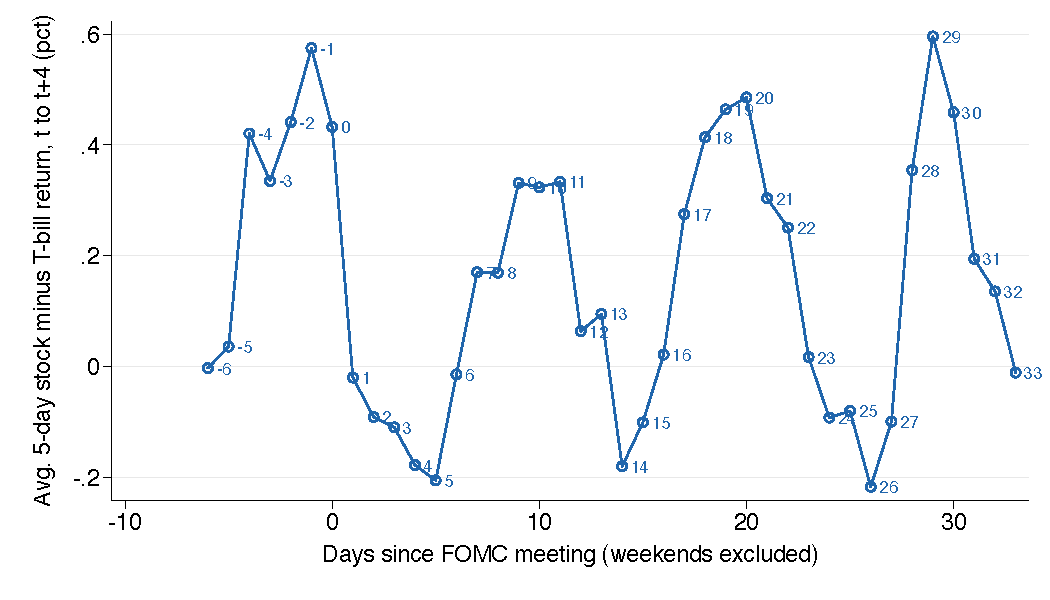
\includegraphics[width=0.7\textwidth]{figures/cies19/fig1}
    \caption{cies19 - Fig1}
\end{figure}


The authors present three distinct trading strategies (A, B, and C) that shed light on the influence of the FOMC cycle on stock market returns. Of particular note is Strategy A, which involves exclusively holding stocks during even FOMC cycle weeks, a strategy conveniently implementable through Exchange-Traded Funds (ETFs). This strategy demonstrates that the average annual returns more than double compared to holding an ETF throughout the entire FOMC cycle. Intriguingly, the authors find that holding an ETF during uneven FOMC weeks results in financial losses over the examined period from 1994 to 2016.
The authors extend their analysis to explore whether the FOMC cycle return pattern extends beyond the United States, potentially influenced by movements of the dollar currency. To investigate this, they use ETFs containing globally diversified stocks. To establish causality, the authors compare FOMC cycles with other macroeconomic news calendars (e.g. Bloomberg macroeconomic news), dispelling the notion that macroeconomic news significantly correlates with FOMC cycle calendars. They also provide evidence that the release of quarterly firm profits does not substantially account for the observed equity premium patterns over the FOMC cycle.
To establish a causal link between the FEDs policy measures and stock market behavior, the authors study intermeeting target changes, Fed funds futures, and internal Board of Governors meetings. 
The authors suggest significant influence by the FED over the stock market through its accommodating policies, leading to reductions in the equity premium. Moreover, they argue to uncover evidence of systematic informal communication channels between Fed officials and the media and financial sector, serving as a channel through which news about monetary policy has reached the market.

\section{The Economics of the FED Put}

The follow-up paper The economics of FED put” by \parencite{cieslak_economics_2021}“ further tries to study the economics of the relationship between FED policy and the stock market. 
The authors compare the stock market as predictive power to other economic indicators to predict changes of the Federal Funds Rate (FFR) by using textual analysis from former Federal Open Market Committee (FOMC) meeting transcripts.
Their findings affirm the FED indeed pays a lot of attention to the stock market during market downturns.

\begin{figure}[h]
    \centering
    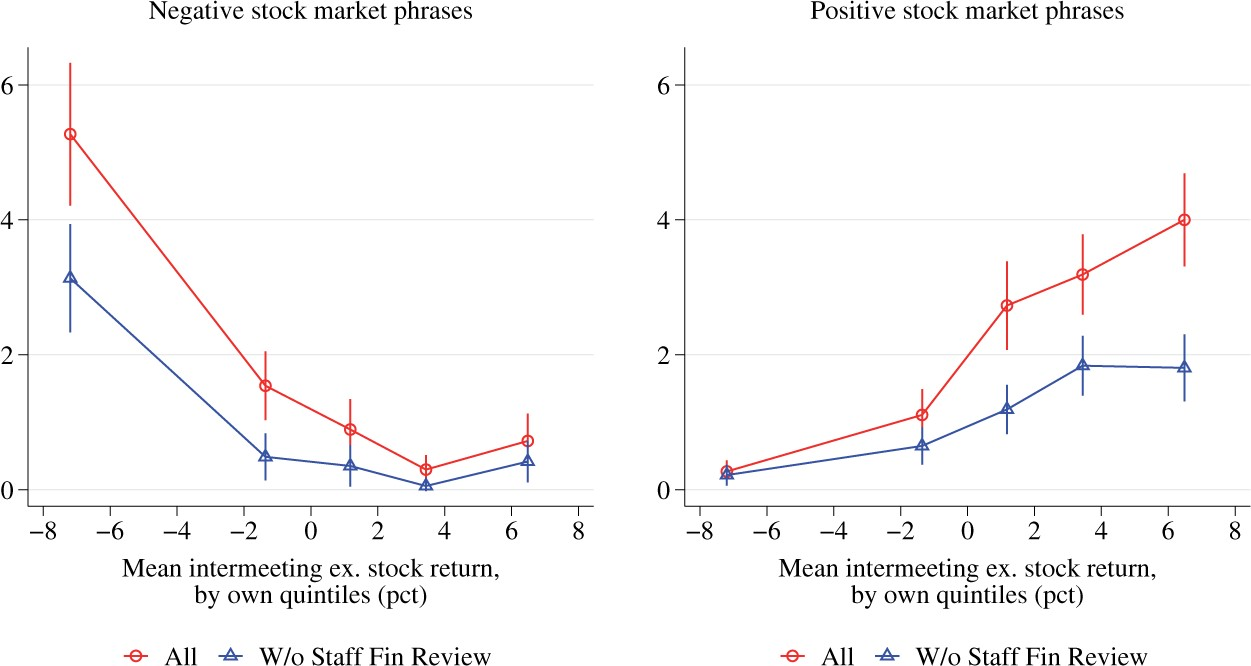
\includegraphics[width=0.7\textwidth]{figures/cies21/Figure6}
    \caption{cies21 - Fig6}
\end{figure}


They argue that the fed put is fueled by the Federal Reserve's concerns about the consumption wealth effect. Conversely, a strong stock market performance corresponds to updates of the FED’s internal growth projections.
Empirical evidence substantiates their claims, as multiple regressions on changes in the Federal Funds Rate (FFR) demonstrate that the stock market captures a higher proportion of the variance (R-squared) compared to other macroeconomic indicators. Significantly, this relationship appears to be less pronounced before the 1990s period.
During the third European Central Bank (ECB) research conference, valuable comments on the econometric approach used by the authors were made by the discussant.

 Emmanuel Moench, the former head of research at Deutsche Bank. Moench's suggests that the correlation between negative stock excess returns and the Federal Funds Rate is heavily influenced by two specific FOMC meetings (during financial crises like the dot-com bubble burst in 2001 and the 2008 financial crisis).
Furthermore, he recommended incorporating additional covariates, including consumer confidence news and credit spreads, into the regression models to enhance their explanatory power. Moench sees the stock market as one of several co-factors influencing Federal Reserve policy (presumably over the updates of the FEDs growth projections as stated by the authors), rather than a dominant driver of the FEDs policy.




\chapter{Does the stylized fact of stock excess returns are mainly achieved in FOMC even weeks (0,  2,  4,  6) from 2016 onwards still persist?}



Empirical part I

TODO: Explain how the FOMC cycle time is defined.

TODO: Explain the one of the main regression models used in the paper "Stock Returns over the FOMC Cycle" \parencite{cieslak_stock_2019}

\begin{equation}
	rx_{i}=\hat{\beta_{0}}+D_0*\hat{\gamma_{1}}+D_1*\hat{\gamma_{2}}+\epsilon_i
\end{equation}
where
\begin{equation}
    D_0=
    \begin{cases}
      1, & \text{if in the 0 week within FOMC cycle time. }\\
      0, & \text{otherwise}
    \end{cases}
\end{equation}
and
\begin{equation}
    D_1=
    \begin{cases}
      1, & \text{if in the 2,4 or 6 week within FOMC cycle time. } \\
      0, & \text{otherwise}
    \end{cases}
\end{equation}


Interpret regression results in  \parencite{cieslak_stock_2019}

Line340 replication code add:
"esttab using "Out.tex", stats(N) b(a3) starlevels(*  0.10 ** 0.05 *** 0.010) label nogaps nonote"

{


\ref{table_cies19_1}
\begin{table}
\begin{center}
\begin{adjustbox}{width=1\textwidth}
%%% estout toutput:
\def\sym#1{\ifmmode^{#1}\else\(^{#1}\)\fi}
\begin{tabular}{l*{3}{c}}

\hline\hline
                    &\multicolumn{1}{c}{(1)}&\multicolumn{1}{c}{(2)}&\multicolumn{1}{c}{(3)}\\
                    &\multicolumn{1}{c}{1-day excess return, day t, pct}&\multicolumn{1}{c}{1-day excess return, day t, pct}&\multicolumn{1}{c}{1-day excess return, day t, pct}\\
\hline
Dummy=1 in Week 0   &       0.174*  &       0.136***&      0.0754*  \\
                    &      (1.92)   &      (2.76)   &      (1.78)   \\
Dummy=1 in Week 2,4,6&       0.176***&      0.0993***&      0.0674*  \\
                    &      (2.67)   &      (2.65)   &      (1.68)   \\
Constant            &     -0.0488   &     -0.0210   &     0.00401   \\
                    &     (-1.15)   &     (-0.96)   &      (0.19)   \\
\hline
N                   &         783   &        5214   &        2937   \\
\hline\hline

\end{tabular}
%%%
\end{adjustbox}
\caption{\label{table_cies19_1}TODO: add a caption here.}
\end{center}
\end{table}

}




TODO: Use the regression model to estimate variable for a newer timeframe from 2016 onwards.

\chapter{Is there empirical evidence for a similar effect when considering only the euro-zone and euro-zone stock returns.  Does it imply an equivalent of the Fed Put in the Euro-Zone?}

Empirical part II

Substitute for euro-zone stock excess returns as regressor variable.

Also regress on "ECB policy meetings calendar week". 

* Can anything be learned/infered from the new regressions? -> Probably not really.
* Low R2, missing controls/covariates, missing domain specific knowledge, etc.
* causal mechanism?
* How much do 2 specific events excluded from the results change the regression results?
* Any implications???


\chapter{Conclusion}

Conclusio / Implications / Further Notions





%%%%%%%%%%%%%%%%%%
\printbibliography

%%%%%%%%%
\appendix

\end{document}